\section{Motivation}\label{motivation}

\emph{This section is co-authored with Marissa Allen}

\begin{figure}[htbp]
\centering
\includegraphics{figures/shared/02_Overview/allcards.pdf}
\caption{A sample of cards created using Foldlings. For larger images
and fold patterns, see \nameref{appendix-d-sample-cards} on page
\pageref{appendix-d-sample-cards}.}
\end{figure}

We set out to create a tool that would help people design 3D pop-up
cards. We were driven by the desire to create original kirigami designs
without a template. As we progressed in our project, we began to focus
on developing a tool that would provide a way to create pop-ups more
intuitively, without explicitly understanding how to create a valid
90-degree pop-up card. Our tool allows users to design, iterate, and
preview an original pop-up card before they even pick up a pair of
scissors.

We outline some user stories --- potential use cases for our software:

\begin{itemize}
\itemsep1pt\parskip0pt\parsep0pt
\item
  George is an avid scrapbooker. He uses Foldlings to create small
  pop-up elements to liven up his scrapbooks. Sometimes he, creates
  cards to commemorate moments --- other times, he pastes photos or
  other media onto a pop-up card structure created with our app.
\item
  Sally designs cards for a commercial greeting card company. She uses
  Foldlings to create rough prototypes and concept sketches for pop-up
  cards. After getting feedback from the rest of her team, she brings
  the exported SVG file into Adobe Illustrator to refine the final card
  designs.
\item
  Jim forgot to make a card for his wife's anniversary present, and
  she's coming home in an hour! He downloads Foldlings from the Apple
  App Store, and is able to quickly design and create a beautiful card.
\item
  Alex is a creative college student who wants to continue making things
  for her friends and family. She wants to explore pop-up cards, but
  doesn't like any of the templates she's found online and can't pay for
  pop-up design books. She finds Foldlings in the Apple App Store and
  tests her creativity with our tool.
\item
  Kate, a middle school math teacher, is teaching a module on pop-up
  card geometry. She uses Foldlings to teach the students about the
  parallelogram constraints between planes as cards fold. By using our
  app, her students gain an intuitive understanding of the geometric
  constraints.
\end{itemize}

\section{Technical Overview}\label{technical-overview}

\emph{This section is co-authored with Marissa Allen}

Our algorithmic simulation and validity detection is based on a tight
set of constraints to the pop-up card problem. We require the card to
have a central main valley fold --- from there we can determine the
orientation, as alternating folds fold in opposite orientations. The
card then folds 180 degrees; this implies parallelogram constraints
between all the edges in a sideways cross-section (with the exception of
v-fold features).

We capture touch input, translating touches into cuts and folds
depending on the geometry of the fold feature. We validate fold features
before they are added to the sketch, ensuring that the design can fold
in 3D. At this point, we also perform bezier path operations to modify
existing edges in the sketch based on the new design element. When a
fold feature is added to the sketch, we re-calculate planes (areas
enclosed by cuts and folds) by traversing a directed graph of edges in
the sketch. Based on these 2D planes, we create 3D planes, which are
oriented and translated based on their relationship to other planes in
the sketch. In 3D, we animate planes in response to user input. Each of
the planes is translated in relation to the plane oriented above the
fold and rotated in relation to the main driving joint.

Our approach constructs a tree representation of the planes based on
fold adjacency and uses this for determining the parent child
relationships in the simulated 3D view. We also use a tree-based
structure to store associations between logical geometric units.

\subsection{Development Process}\label{development-process}

\begin{figure}[htbp]
\centering
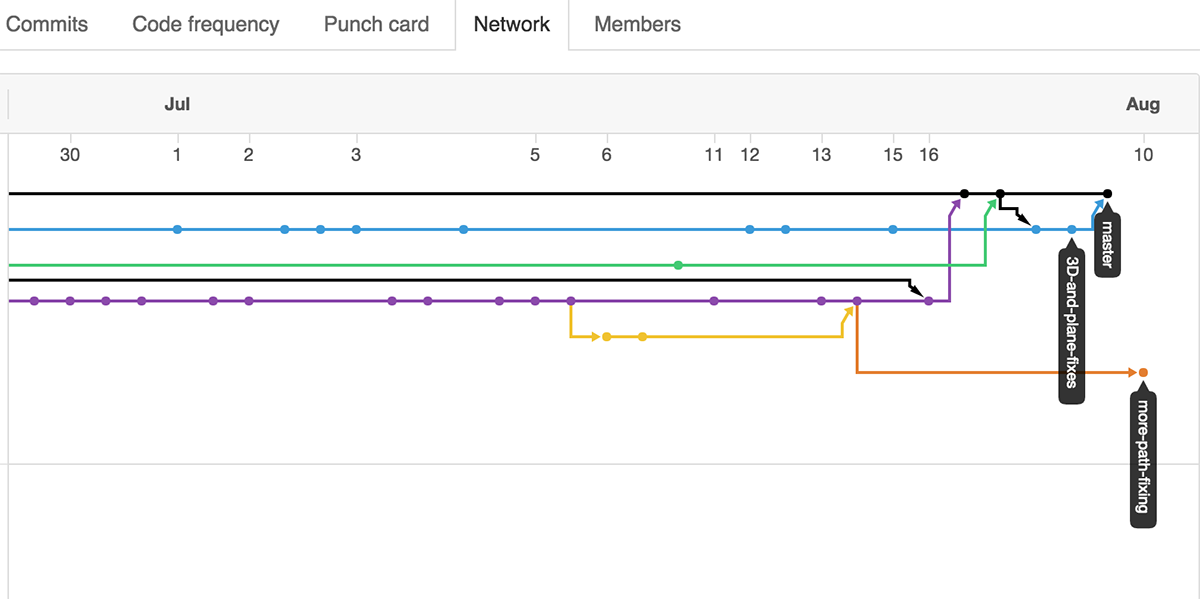
\includegraphics{figures/shared/02_Overview/gitflow.png}
\caption{Branches in our github.com repository.}
\end{figure}

We designed and developed the software interactively, frequently testing
prototypes with users. We used github to build Foldlings
collaboratively. Our workflow involved creating new code branches for
each feature, and reviewing the changes before merging back into the
master branch of the codebase. The full source for our software is
available at \url{http://github.com/harquail/foldlings/}.

\section{Pipeline Overview}\label{pipeline-overview}

\emph{This section is co-authored with Marissa Allen}

\begin{figure}[htbp]
\centering
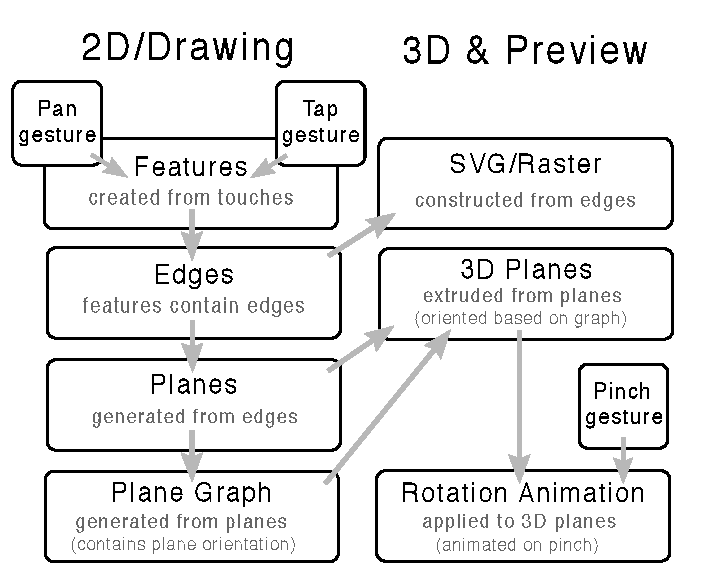
\includegraphics{figures/shared/02_Overview/pipeline.pdf}
\caption{Overview of data flow between 2D and 3D systems.}
\end{figure}

To begin, a user draws a design using the fold feature tools: box fold,
polygon, freeform and v-fold. These tools create a pattern of cuts and
folds, displaying an interactive preview of the design as the user
creates it. The cuts and folds created with these tools remain
associated with each other, and can be modified or deleted as a unit.

Each time a new shape is added to the design, it is evaluated for
validity: whether it can fold to 90 degrees and be parsed into
individual planes. The planes are then linked together in an acyclic
graph based on the planes' abutting top edges. This acyclic graph allows
us to shade planes based on orientation in 2D and simulate the design in
3D. Each feature can also be modified or deleted, by tapping on the
feature an selecting an entry from the list of available options.

This process continues until the user previews the design in 3D. The 3D
preview displays a simulation of how the design will fold, which can be
manipulated using a pinch gesture. The user is free to return to the 2D
drawing interface and continue editing his/her design or save the design
as either a raster file or SVG vector file. After this step, the user
can print and cut the raster file or open the SVG file on a laser cutter
or other cutting tool. We automatically save designs locally when
leaving the design workspace, so users can restore their work.

Figure 1.6 shows the full pipeline for designing cards. It shows a
user's design process, starting with concept sketches, and moving
through iterations of the sketch using 3D preview to test the design.
Finally, the user exports the design as a fold pattern, and cuts and
folds the pop-up card.

\begin{figure}[htbp]
\centering
\includegraphics{figures/shared/02_Overview/sinewave.pdf}
\caption{A full outline of the design process for our application, from
initial concept sketches to full realization of a paper pop-up card.}
\end{figure}
